\documentclass{article}
\usepackage{enumerate}
\usepackage{amsmath}
\usepackage{tikz}
\usetikzlibrary{arrows,positioning} 

\setlength{\parindent}{0.0in}
\setlength{\parskip}{0.1in}

\title{Methods in Artificial Intelligence \\
        \normalsize Exercise 1}
\author{Herman Schistad - MTDT}
\date{13.01.2012}
\begin{document}
\maketitle

\section*{5-card Poker Hands}
Considering the domain of the 5-card poker hands from a standard deck of 52 cards. Assuming the dealer is fair.
\begin{enumerate}[(i)]
\item How many atomic events are there in a joint probability distrubution?

The joint probability distrubution is:
\begin{equation}
{52 \choose 5} = 2,598,960
\end{equation}

\item What is the probability of each atomic event?

The probability of a single event is given by:
\begin{equation}
P(x) = \frac{Wanted}{Total}
\end{equation}

A single atomic event is then, by (2), given: 
\begin{equation}
P(x) = \frac{1}{2,598,960} = .000000385
\end{equation}

\item What is the probability of being dealt a {\bf royal straight flush}?

In order to calculate a the probability of a royal straight flush we first select the suit, and this card needs to have a value of 10 or higher - therefore, in order to select the first card corectly,  we have the probability of:
\begin{equation}
P(x) = \frac{20}{52}
\end{equation}

When we have selected our suit, we need to stick with this and now for the rest of the remaining 4 cards:
\begin{equation}
P(x) = \frac{4}{51} \cdot \frac{3}{50} \cdot \frac{2}{49} \cdot \frac{1}{48}
\end{equation}

Finally we combine (4) and (5) and calculate the probabilty for a royal straight flush (RSF):
\begin{equation}
P(RSF) = \frac{20 \cdot 4 \cdot 3 \cdot 2 \cdot 1}{52 \cdot 51 \cdot 50 \cdot 49 \cdot 48} = \frac{480}{311,875,200} = .000154
\end{equation}

We could also derive this answer by looking at how many royal-straight-flushes which are possible in grand total. The answer here is a total of 4 different royal straight flushes. By (i) we can get the probability:

\begin{equation}
P(RSF) = \frac{4}{2,598,960} = \frac{1}{649740} = .000154
\end{equation}


\item What is the probability of being dealt {\bf three of a kind}?

Distrubution of 'Three of a kind' (TOK) is calculated by counting total number of possible hands and then dividing this on total hands possible in a 5-card shuffle.
\begin{equation}
P(TOK) = \frac{\binom{13}{1} \cdot \binom{4}{3} \cdot \binom{12}{2} \cdot \binom{4}{1} \cdot \binom{4}{1}}{2,598,960} = \frac{54,912}{2,598,960} = .021128451
\end{equation}
\end{enumerate}

\newpage
\section*{Bayesian Network Construction}

I've drawn a Bayesian network showing {\bf my interpreation} of the different states given in the task.
Each box/node has different states inside, with a given probability.

As I interpret this task there is no 100\% correct answer, but, depending on how you view the world and the society a variety of different solutions. I therefore chose the relations I found most probable. \\

\tikzset{
    %Define standard arrow tip
    >=stealth',
    %Define style for boxes
    box/.style={
           rectangle,
           rounded corners,
           draw=black, very thick,
           text width=10em,
           minimum height=2em,
           text centered},
    % Define arrow style
    arrow/.style={
           ->,
           thick,
           shorten <=2pt,
           shorten >=2pt,}
}

\begin{figure}[h]
\centering
\begin{tikzpicture}[node distance=0.6cm, auto,]
  \node[box] (illness) {Illness at the moment};
  \node[box, above=of illness] (history) {History of illness}
    edge[arrow] (illness.north);
  \node[above=of history] (dummy) {};
  \node[box, right=of dummy] (fish) {Fish-eating habits}
    edge[arrow, bend left=20] (history.east);
  \node[box, left=of dummy] (fiber) {Fiber-eating habits}
    edge[arrow, bend right=20] (history.west);
  \node[box, above=of dummy] (income) {Household-income}
    edge[arrow, bend left=20] (fish.north)
    edge[arrow, bend right=20] (fiber.north);
  \node[box, above=of income] (drinking) {Drinking habits}
    edge[arrow, <-] (income.north);
  \node[box, above=of drinking] (children) {Number of children}
    edge[arrow] (drinking.north);
  \node[right=of children] (dummy2) {};
  \node[box, left=of children] (religion) {Religion}
    edge[arrow, bend right=20] (drinking.west);
  \node[box, above=of children] (working) {Working parents}
    edge[arrow] (children.north)
    edge[arrow, bend left=45] (drinking.east)
    edge[arrow, bend left=70] (income.east);
\end{tikzpicture}
\caption{Household Bayesian Network - Showing the authors personal interpretation of the different dependencies in the given world. }
\end{figure}

\newpage

In this figure 'Illness at the moment' is conditionally independent on 'fiber-eating habits', 
and 'fish-eating habits' given 'history of illness'. One could also argue that drinking
habits would affect the history of illness, and in that case 'Illness at the moment' would be conditionally
independent of 'number of children', 'working parents' and 'religion' given 'driking habits'. 

We also note that given 'household income' the 'fiber-eating habits' and 'fish-eating habits' becomes
independent. If we are given 'history of illness' we see, however, that the 'fish and fiber-eating habits' are dependent. This makes sense if we consider that the 'history of illness' is unknown and therefore 
'fish and fiber-eating habits' are dependent. The same as we saw when we do not know 'household income'!

When neither 'religion', 'number of children', 'drinking habits' nor 'working parents' are known we say
that they are all independent. However if we know 'driking habits' they all become dependent.

I find these results to be reasonable as they depict a good simultation of a real world. One could of course
argue that we have more dependencies (e.g. refer to the 'Butterfly effect' which states that all events are dependent) but as an illustration of the Bayesian Network this gives us a general idea.

One could however also argue that e.g. even though 'fish and fiber-eating habits' are independent given 'household income', a good income would produce a person which ate fibers and fish (which are expensive) and if 
one eats a lot of fish/fiber it is reasonable to think that one eats a lot of the other too (and they are in
fact dependent)

\newpage
\section*{Bayesian Network Application}

{\bf Yes, you should change the door}. Why?

When you first select a door, it has 1/3 probabilty of containing a prize - and the probability for losing is 2/3. 
When the official then opens a door he eliminates one of the doors which initially was wrong. 
\\ Now, if you change you will win 2/3 of the times (since this was the probability for one of the other doors was correct, before the official opened it)

Confusing? Let's look at the bayesian network to clear things up; The Bayesian Network corresponding to the Monty Hall Problem, which is essence is the same problem as depicted in the given assignment has the following dependencies: \\

\begin{figure}[h]
\centering
\begin{tikzpicture}[node distance=0.6cm, auto,]
  \node[box] (openedByOfficial) {Opened By Official};
  \node[box, left=of openedByOfficial] (myChoice) {My Choice}
    edge[arrow] (openedByOfficial.west);
  \node[box, right=of openedByOfficial] (prize) {ContainsPrize}
    edge[arrow] (openedByOfficial.east);
\end{tikzpicture}
\caption{The Bayesian Network corresponding to the Monty Hall Problem. }
\end{figure}

I visualized this is GeNie (Graphical Network Interface) by adding a 'decision node' (myChoice) and two 'chance nodes' (openedByOfficial and ContainsPrize). 
The probability/chance of a door containing a prize is initially 1/3 for A, B and C - and this is entered in the node properties of ContainsPrize.

In the OpenedByOffical we applied the following node properties:

\begin{table}[h]
    \begin{tabular}{|l|l|l|l|l|l|l|l|l|l|} 
    \hline
        ContainsPrize & \multicolumn{3}{|c|}{A} & \multicolumn{3}{|c|}{B} & \multicolumn{3}{|c|}{C} \\ \hline
        MyChoice      & A   & B & C & A & B   & C & A & B & C   \\ \hline
        openA         & 0   & 0 & 0 & 0 & 0.5 & 1 & 0 & 1 & 0.5 \\
        openB         & 0.5 & 0 & 1 & 0 & 0   & 0 & 1 & 0 & 0.5 \\
        openC         & 0.5 & 1 & 0 & 1 & 0.5 & 0 & 0 & 0 & 0   \\
    \hline
    \end{tabular}
    \caption{The definitions given to GeNie in the 'Opened By Official' node}
\end{table}

\newpage
If one then set the decision on 'MyChoice' to A, set the evidence on ContainsPrize to A and make the official open the door B - we achieve the following probabilites in GeNie:

\begin{figure}[h]
\centering
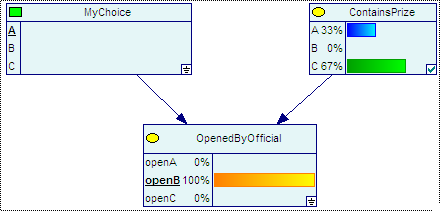
\includegraphics[scale=0.75]{genieresult.png}
\caption{The visualization result in GeNie}
\end{figure}

Notice this rather impressive result! If the official shows you a door which does not contain a prize (which he will) you have a 67\% chance of winning by changing your door to C, rather than staying where you are.

This may seem 'unlogical' as many only observe the world 'as-is' without taking into the account the huge hint given by the offical.
Therefore one is lead to believe that the probability of winning is now 50\% since you have two options. But by using the
{\bf Bayesian Rule} we have showed that this in fact is not the case.

\end{document}
